\documentclass[a4paper]{article}
\usepackage[utf8]{inputenc} % accents xuten bé
\usepackage[T1]{fontenc} % també pels accents, meh
\usepackage[catalan]{babel} % idioma
\usepackage{titlesec} % per a canviar format dels títols
\usepackage{titling} % per a poder definir \subtitle
%\usepackage[none]{hyphenat} % no separa paraules
\usepackage{mathtools} % millor que amsmath (opcions de notació mates)
\usepackage{amsfonts} % segurament per definir = amb coses dalt
\usepackage{cases} % per poder fer les típiques definicions per parts de funcions amb corxets
\usepackage{blindtext} % textos de prova, tipus loremipsum
\usepackage{enumitem} % llistes
\usepackage{geometry} % per controlar els marges
\usepackage{indentfirst} % per controlar la indentació de la primera línia de cada paràgraf
\usepackage{physics} % sobretot, derivades (parcials)
\usepackage{xcolor} % colors
\usepackage{float} % per controlar posicions de flotants (imatges i taules)
\usepackage{hyperref}
\usepackage{multirow}
\usepackage[per-mode=symbol]{siunitx}
\usepackage{graphicx}
\usepackage{caption}
\usepackage{subcaption}
%\usepackage{biblatex}
%\usepackage[
%backend=biber,
%style=alphabetic,
%citestyle=authoryear
%]{biblatex}

\usepackage{graphicx} % alguna cosa per a imatges
\graphicspath{ {./images/} }

% Que la primera línia no estigui indentada
\setlength{\parskip}{3pt}
\setlength{\parindent}{0cm}

%\titlelabel{\llap{\thetitle\quad}} % No indentació dels títols

%Marges
%\hoffset = 0in
%\oddsidemargin = 13pt
%\textwidth = 427pt

%Comandes útils
\newcommand\eqdef{\mathrel{\overset{\makebox[0pt]{\mbox{\normalfont\tiny\sffamily def}}}{=}}}
\newcommand\eqimp{\mathrel{\overset{\makebox[0pt]{\mbox{\normalfont\tiny\sffamily imp}}}{=}}}
\newcommand\eqtext[1]{\mathrel{\overset{\makebox[0pt]{\mbox{\normalfont\tiny\sffamily {#1}}}}{=}}}
\renewcommand\vnabla{\vec{\nabla}}
\newcommand\vecv{\vec{v}}
\newcommand{\vvec}[1]{\vec{\vec{#1}}}
\newcommand\vecdot[1]{\dot{\vec{#1}}}
\newcommand\redtext[1]{\textcolor{red}{#1}}
\newcommand{\ten}[2]{\ensuremath{{#1}\times 10^{#2}}}
\DeclareMathOperator\arctanh{arctanh}

% definició de \subtitle
\newcommand{\subtitle}[1]{%
  \posttitle{%
    \par\end{center}
    \begin{center}\large#1\end{center}
    \vskip0.5em}%
}

\setlength{\droptitle}{-6em} 

% Format dels títols
\titleformat*{\section}{\Large\bfseries}
\titleformat*{\subsection}{\bfseries}

\captionsetup{
    width=\textwidth, % width of caption is 90% of current textwidth
    labelfont=bf,        % the label, e.g. figure 12, is bold
    font=small,          % the whole caption text (label + content) is small
%    format=hang,         % no caption text under the label
}

% Si funcionés, algun format de pàgina
%\pagestyle{fancy}
%\fancyhf{}
%\rhead{Share\LaTeX}
%\lhead{Guides and tutorials}
%\rfoot{Page \thepage}

% AND HERE WE GO

\title{\textbf{Simulació 2D del Model d'Ising}}
\subtitle{\scshape{Fenòmens col·lectius i transicions de fase}}
\author{Ivan Alsina Ferrer}
\date{}

\begin{document}

\maketitle
\vspace{-4em}
\section{Introducció}

El model d'Ising té una importància cabdal en física estadística perquè proporciona una sèrie de tècniques matemàtiques per a treballar amb xarxes $n$-dimensionals de partícules que permeten entendre el comportament crític d'una gran varietat de sistemes a la natura. L'hamiltonià que proporciona és el següent:
\begin{equation} \label{ising_hamiltonian}
    \mathcal{H}^* \equiv \mathcal{H}/J = -\sum_\text{nn} \sigma_i \sigma_j - \frac{B}{J} \sum_{i=1}^{N} \sigma_i
\end{equation}
on $\mathcal{H}^*$ és l'hamiltonià reduït, és a dir, en unitats de l'energia d'interacció entre les partícules $J$. nn fa referència a \textit{nearest neighbors}, o \textit{primers veïns}, indicant que el sumatori involucrat s'extén sobre les parelles de partícules que estan a distància mínima. $B$ és el camp aplicat, en unitats de $\mu$, però en el nostre cas no en considerarem el terme ja que l'estudi ha estat considerant camp nul.

El treball que presentem estudia un sistema bidimensional d'$N$ partícules, distribuïdes segons una matriu $L\times L$, i descrites per un spin, representat com a $\sigma_i$ en l'equació \eqref{ising_hamiltonian}. Aquest pot estar orientat en dues direccions: bé amunt (valor $+1$) o avall (valor $-1$). L'estat fonamental d'aquest sistema, quan es troba a una temperatura fixada, minimitza l'energia lliure de Helmholtz.
\begin{equation*}
    F = U - TS
\end{equation*}
Per a fer-ho, pot minimitzar l'energia interna $U$ o bé maximitzar l'entropia $S$. Un sistema a baixa temperatura mostra el primer comportament, i es diu que està en la seva fase ordenada. Un sistema a alta temperatura, en canvi, té preferència pel segon, mostrant-se en la seva fase desordenada. El pas d'un comportament a l'altre constitueix una transició de fase i és el que estudiarem amb detall en el present treball tot descrivint el comportament de les propietats termodinàmiques prop de la temperatura a què això té lloc, la temperatura crítica o de Curie ($T_c$).

Per a dur a terme aquest estudi, havent partit d'una configuració aleatòria d'spins, hem emprat l'algorisme de Metròpolis amb què, valent-se d'un gran nombre d'iteracions Montencarlo, s'han explorat les cadenes de Markov que descriuen el sistema. En cadascuna d'aquestes iteracions, s'han fet $N$ propostes de canvi d'spin, de manera aleatòria. Les propostes que suposen una disminució de l'energia s'accepten, i aquelles, en canvi que, suposen un augment de la mateixa, s'accepten amb probabilitat $\exp\left(-\Delta E^*/T^*\right)$. Això es tradueix en una penalització als canvis en spin que augmenten l'energia del sistema si l'increment es gran o si la temperatura a què es donen és baixa. Repetint el procés per a diferents llavors per a assegurar una bona exploració de l'espai de configuracions, s'han calculat les mitjanes amb què després s'han trobat les propietats termodinàmiques d'interès. Aquest procediment s'ha fet per a valors de temperatura reduïda en un rang de 1.5 a 3.5, i per a sistemes de longitud $L=15,30,45,60,75,90,120$.

Amb les dades resultants s'han explicat el comportaments de l'energia, capacitat calorífica, imantació i susceptibilitat monoparticulars del sistema, i se n'ha trobat la temperatura crítica. A més, ha estat possible una descripció del comportament d'aquestes propietats en el veïnatge de la mateixa.

\section{Evolució d'imantacions i temperatures}

L'algorisme de Metropolis que tot just hem descrit s'ajusta a la naturalesa probabilística de les fluctuacions en l'energia i la imantació dels sistemes termodinàmics. És per aquest motiu que, tot i no haver definit una dinàmica pròpia del sistema, podem argumentar que les iteracions Montecarlo en la simulació donen una noció de l'evolució temporal d'un sistema que, partint d'una configuració inicial aleatòria (en el nostre cas, determinada per la llavor que fem servir), es veu sotmès a una temperatura donada. Veiem l'evolució d'aquestes magnituds al llarg de les iteracions, per a diferents temperatures:


\begin{figure}[H]
    \centering
    \begin{subfigure}{.49\textwidth}
        \centering
        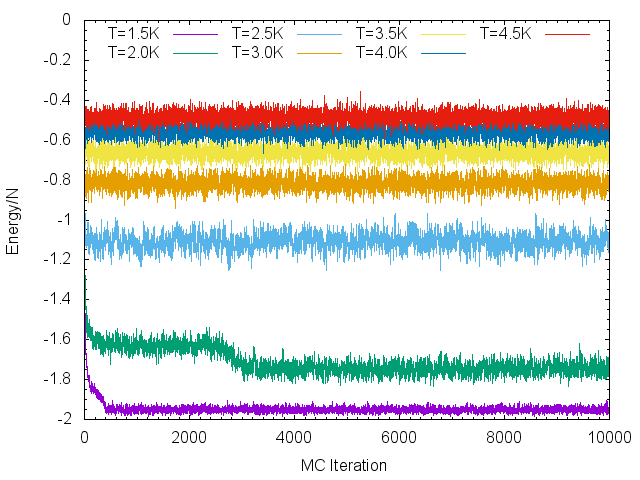
\includegraphics[width=\textwidth]{SIM-L-060-energy-EVO.png}
        \caption{Energies per partícula}
        \label{fig:evo_ene}
    \end{subfigure}
    \begin{subfigure}{.49\textwidth}
        \centering
        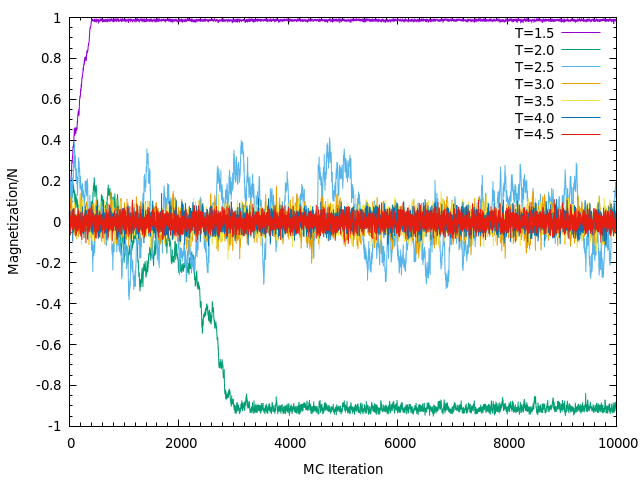
\includegraphics[width=\textwidth]{SIM-L-060-magnetiz-EVO.png}
        \caption{Imantacions per partícula}
        \label{fig:evo_mag}
    \end{subfigure}
    \caption{Evolució de les energies per partícula i les imantacions per partícula al llarg de les iteracions Montecarlo, per a temperatures reduïdes $T^*$ en el rang 1.5 a 4.5, en un sistema quadrat de $L=60$ spins de costat.}
\label{fig:evo}
\end{figure}

Tal com veiem a la figura \ref{fig:evo_ene}, per a temperatures baixes l'energia per partícula del sistema convergeix ràpidament a 2 cops l'energia de lligam. Això és degut a que, en aquesta situació, com que el sistema minimitza l'energia, la major part de les parelles d'spin seran del mateix tipus i, en conseqüència, al límit,
\begin{equation*}
    E^*/N = \langle \mathcal{H} \rangle / N= -\sum_{\langle{i,j\rangle}} 1/N = -\frac{1}{2}z = -2
\end{equation*}
en què $z$ és el nombre de coordinació ($z=4$) i on recordem, treballem en unitats reduïdes d'energia. A temperatures altes, en canvi, el sistema es troba en la fase desordenada i tendeix a maximitzar l'entropia. Això significa que hi haurà parelles amb el mateix spin i amb spin contrari amb la mateixa probabilitat, provocant que l'energia per partícula sigui, en valor absolut, petita.

En augmentar les temperatures, es pot observar com hi ha una temperatura per la qual la imantació és altament fluctuant (en la figura \ref{fig:evo_mag}, $T^*=2.5$). La raó és que aquesta temperatura és molt propera a la temperatura crítica del sistema i, tal com estudiarem més endavant, les correlacions es fan de molt llarg abast, de tal manera que l'estabilitat de les propietats termodinàmiques del sistema es veuen compromeses.

Presentem a continuació la configuració final del sistema després de 10 000 iteracions Montecarlo a temperatures alta i baixa, de forma que se'n posi de manifest la fase ordenada i desordenada, respectivament.

\begin{figure}[H]
    \centering
    \begin{subfigure}{.45\textwidth}
        \centering
        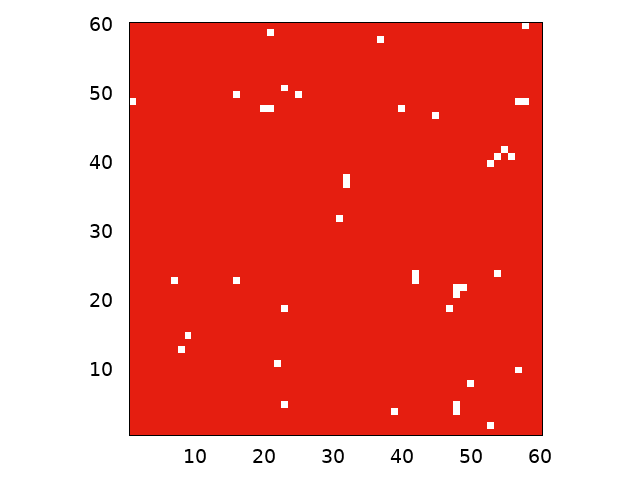
\includegraphics[width=\textwidth]{SIM-L-060-TEMP-1500.png}
        \caption{$T^*=1.5$}
        \label{fig:conf_low}
    \end{subfigure}
    \begin{subfigure}{.45\textwidth}
        \centering
        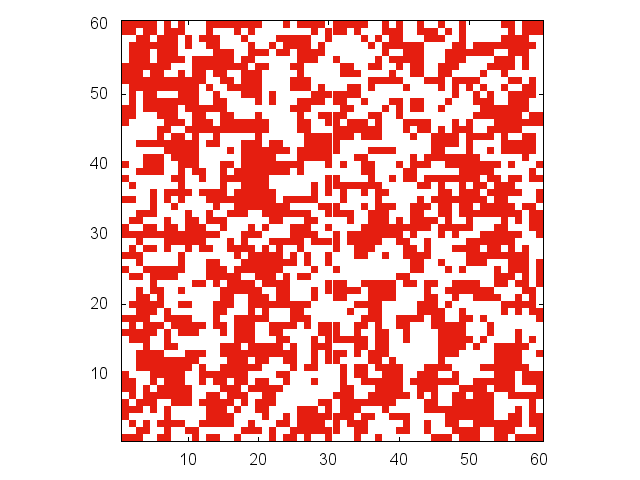
\includegraphics[width=\textwidth]{SIM-L-060-TEMP-4500.png}
        \caption{$T^*=4.5$}
        \label{fig:conf_high}
    \end{subfigure}
    \caption{Configuració final, després de 10 000 iteracions Montecarlo, del sistema amb $L=60$ spins de costat de què se'n mostrava l'evolució a la figura \ref{fig:evo}, per a les temperatures reduïdes $T^*=1.5$ i $T^*=4.5$. Els quadrats vermells representen spins orientats cap amunt. Els blancs, spins orientats cap avall.}
\label{fig:conf}
\end{figure}

La figura \ref{fig:evo} mostra una situació en què s'arriba a la convergència prou aviat, però en general haurem de fer promitjos amb un gran nombre d'iteracions (al voltant d'unes 40 000) per a compensar les fluctuacions estadístiques, i un gran nombre de llavors (al voltant d'unes 120) per a contrarestar el fet que un cop el sistema pren una configuració determinada, és energèticament molt costós allunyar-s'hi gaire. D'aquesta forma, podrem explorar l'espai de configuracions amb comoditat. A això se li suma el fet que a la simulació s'han aplicat condicions periòdiques de contorn (\textit{PBC}), que faciliten el tractament de les vores i suposen gran desavantatge quan el sistema es fa gran, però que per contra pot provocar situacions poc realistes a baixes temperatures on una regió vertical o horitzontal de partícules ofereix una gran resistència a prendre l'spin de l'entorn. Si aquestes regions es trenquen, es veuen salts sobtats en l'evolució de l'energia i la imantació, i el sistema s'acosta a la convergència. En tenim un exemple a la temperatura $T^* = 2.0$ de la figura \ref{fig:evo}, entre les iteracions de Montecarlo número 2000 i 3000. Vegem-ne les configuracions d'spin allà:

\begin{figure}[H]
    \centering
    \begin{subfigure}{.24\textwidth}
        \centering
        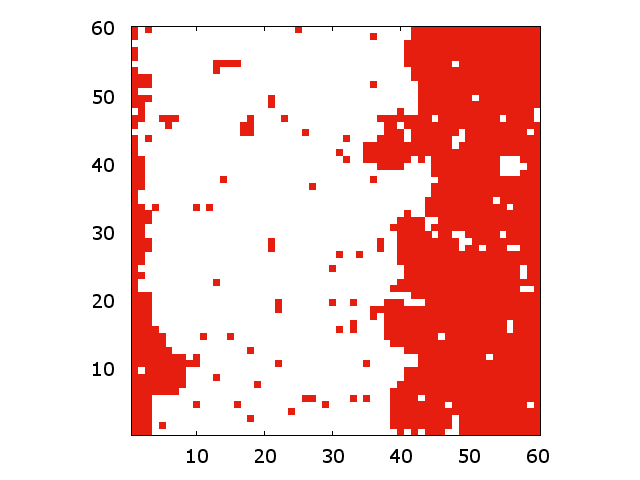
\includegraphics[width=\textwidth]{SIM-L-060-TEMP-2000_40-CEVO.png}
        \caption{Iteració MC 2000}
        \label{fig:conf_2k}
    \end{subfigure}
    \begin{subfigure}{.24\textwidth}
        \centering
        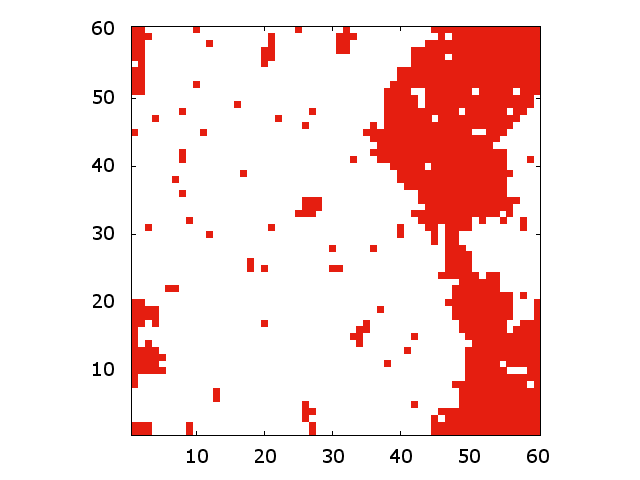
\includegraphics[width=\textwidth]{SIM-L-060-TEMP-2000_52-CEVO.png}
        \caption{Iteració MC 2600}
        \label{fig:conf_2k6}
    \end{subfigure}
    \begin{subfigure}{.24\textwidth}
        \centering
        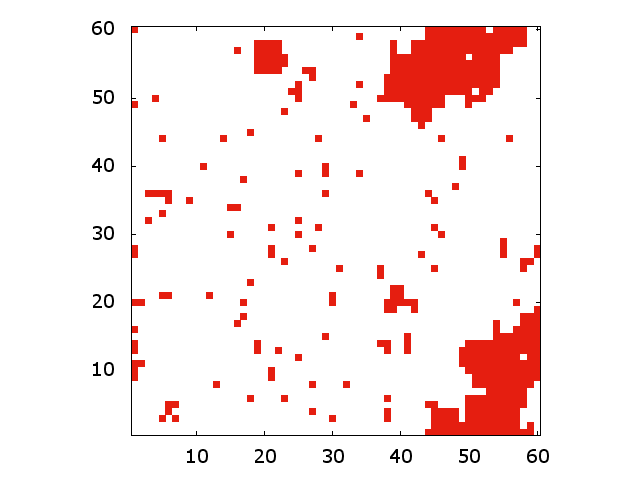
\includegraphics[width=\textwidth]{SIM-L-060-TEMP-2000_56-CEVO.png}
        \caption{Iteració MC 2700}
        \label{fig:conf_2k7}
    \end{subfigure}
    \begin{subfigure}{.24\textwidth}
        \centering
        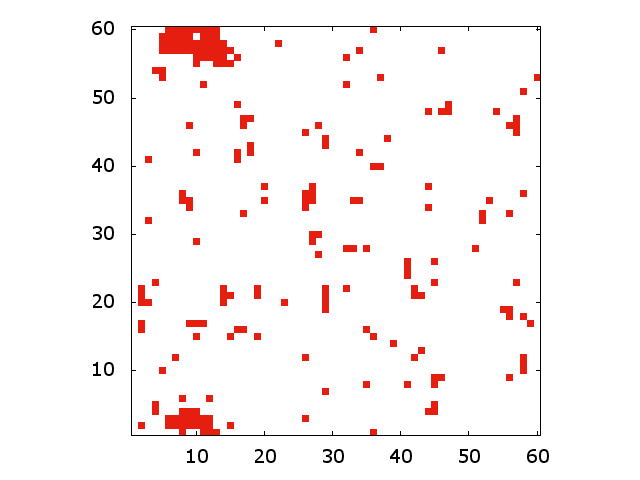
\includegraphics[width=\textwidth]{SIM-L-060-TEMP-2000_60-CEVO.png}
        \caption{Iteració MC 3000}
        \label{fig:conf_3k}
    \end{subfigure}
    \caption{Configuracions d'spin per al sistema de $L=60$, a la temperatura reduïda $T^*=2.0$, entre les iteracions MC 2000 i 3000, en què es produeix el trencament d'una regió que fa convergir ràpidament l'energia i la imantació.}
\label{fig:conf_zoom}
\end{figure}

\section{Magnituds termodinàmiques}

Les magnituds estudiades per a les diferents temperatures són l'energia, capacitat calorífica, imantació i susceptibilitat. Vegem-ne els resultats per a $L=30$:

\begin{figure}[H]
    \centering
    \begin{subfigure}{.45\textwidth}
        \centering
        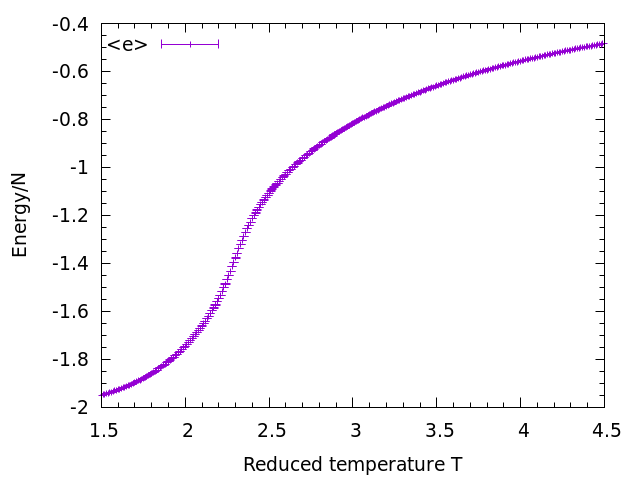
\includegraphics[width=\textwidth]{props-L-030_e.png}
        \caption{Energia per partícula}
        \label{fig:props-e}
    \end{subfigure}
    \begin{subfigure}{.45\textwidth}
        \centering
        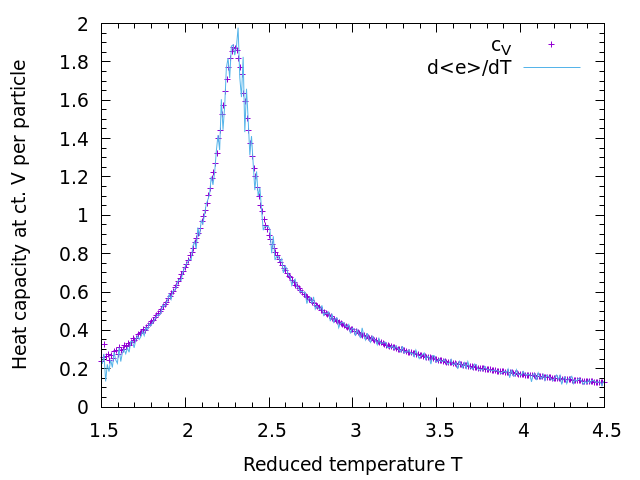
\includegraphics[width=\textwidth]{props-L-030_cvn.png}
        \caption{Capacitat calorífica per partícula}
        \label{fig:props-cv}
    \end{subfigure}
        \begin{subfigure}{.45\textwidth}
        \centering
        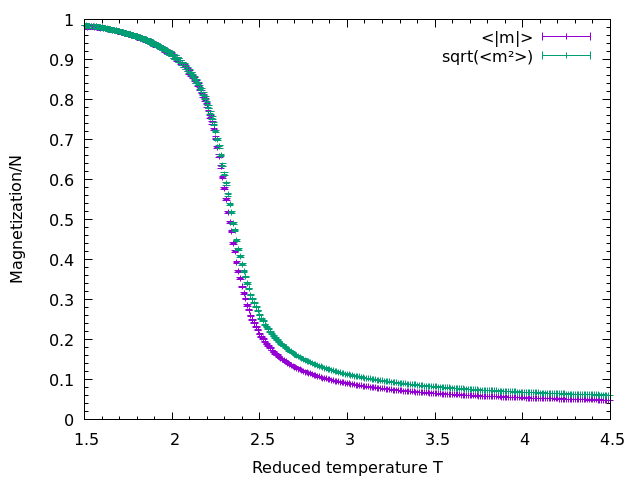
\includegraphics[width=\textwidth]{props-L-030_m.png}
        \caption{Imantació per partícula}
        \label{fig:props-m}
    \end{subfigure}
    \begin{subfigure}{.45\textwidth}
        \centering
        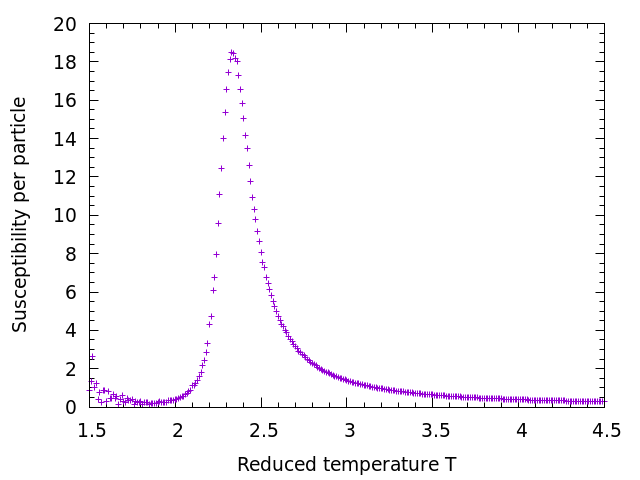
\includegraphics[width=\textwidth]{props-L-030_xn.png}
        \caption{Susceptibilitat per partícula}
        \label{fig:props-x}
    \end{subfigure}
    \caption{Resultats de la simulació per a $L=30$ d'energia, capacitat calorífica, imantació i susceptibilitat, totes les magnituds per partícula. La capacitat calorífica es mostra calculada com la variància de l'energia entre el quadrat de la temperatura, i com la derivada del valor esperat de l'energia respecte de la temperatura. Energia i imantació incorporen barres d'error, preses de la incertesa estadística en les mitjanes.}
\label{fig:props}
\end{figure}

Pel que fa a l'energia (figura \ref{fig:props-e}), podem veure clarament els comportaments asimptòtics comentats en l'apartat anterior: $\langle e \rangle \to -2$ quan $T^* \to 0$, i $\langle e \rangle \to 0$ quan $T^* \to \infty$, que caracteritzen les fases ordenada i desordenada, respectivament. El canvi de règim es dona a la temperatura crítica, on hi té lloc un punt d'inflexió.

Quant a la imantació (figura \ref{fig:props-m}), s'observa un fenomen molt similar, també presentat més amunt. Cal tenir en compte, però, que no podem representar $\langle m \rangle$, vist que com que $m$ pren valors positius i negatius amb igual probabilitat, serà sempre 0 com a conseqüència dels promitjos per a diferents llavors. En comptes d'això, podem mostrar $\langle |m| \rangle$ i $\sqrt{\langle m^2 \rangle}$, indistintament. Ambdós valors esperats tendeixen asimptòticament a 1 per a temperatures petites, i a 0 per a temperatures grans, també descrivint el règim ordenat i desordenat, separats per un punt d'inflexió.

La capacitat calorífica (figura \ref{fig:props-cv}) és una propietat que en el límit termodinàmic té una divergència logarítmica al punt crític. En un sistema amb $L$ finita, però, presenta un màxim al punt crític. Pot calcular-se de dues maneres diferents, que presentem de manera complementària per a comprovar-ne l'equivalència:
\begin{equation*}
    c_V = N \frac{\langle e^2 \rangle - \langle e \rangle^2}{{T^*}^2}, \qquad c_V = \dv{\langle e \rangle}{T^*}
\end{equation*}

Finalment, la susceptibilitat presenta una divergència al punt crític en el límit termodinàmic, que es tradueix en un màxim al punt crític quan simulem un sistema finit.

\section{Efecte de variar la mida}

Un cop hem vist quin és el comportament de les propietats termodinàmiques per a una $L$ determinada, podem representar la dependència de mateixes magnituds amb la temperatura per a les diferents $L$ estudiades.

\begin{figure}[H]
    \centering
    \begin{subfigure}{.45\textwidth}
        \centering
        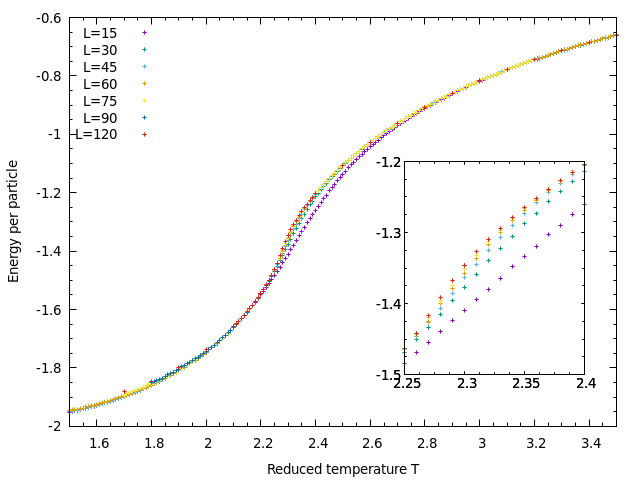
\includegraphics[width=\textwidth]{plot-e.png}
        \caption{Energia per partícula}
        \label{fig:plot-e}
    \end{subfigure}
    \begin{subfigure}{.45\textwidth}
        \centering
        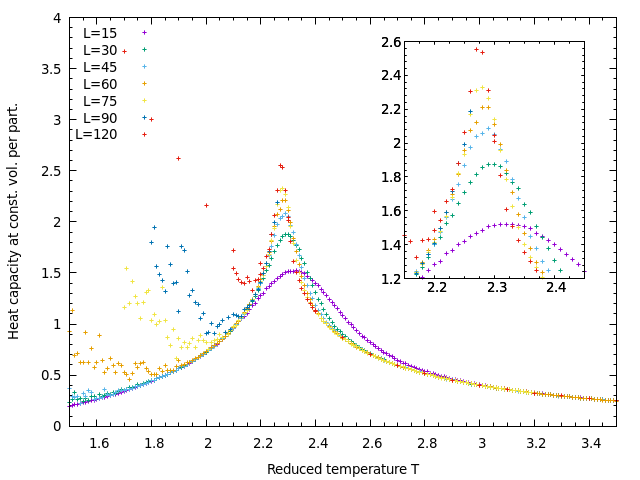
\includegraphics[width=\textwidth]{plot-cv.png}
        \caption{Capacitat calorífica per partíucla}
        \label{fig:plot-cv}
    \end{subfigure}
        \begin{subfigure}{.45\textwidth}
        \centering
        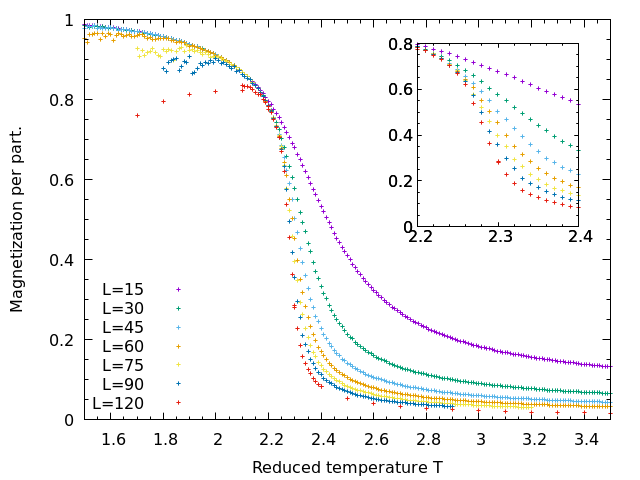
\includegraphics[width=\textwidth]{plot-m.png}
        \caption{Imantació per partícula}
        \label{fig:plot-m}
    \end{subfigure}
    \begin{subfigure}{.45\textwidth}
        \centering
        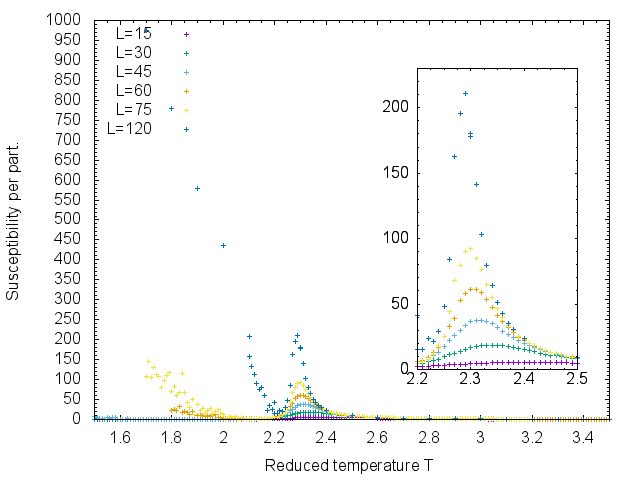
\includegraphics[width=\textwidth]{plot-x.png}
        \caption{Susceptibilitat per partícula}
        \label{fig:plot-x}
    \end{subfigure}
    \caption{Resultats de la simulació de la simulació per a l'energia, capacitat calorífica, imantació i susceptibilitat per a les diferents $L$, totes les magnituds per partícula. Es mostren les regions properes a la temperatura crítica ampliades.}
\label{fig:plot}
\end{figure}

Un fet que es repeteix al llarg de la figura \ref{fig:plot} és que les característiques que són reflex de l'existència d'una temperatura crítica (punts d'inflexió i màxims) van desplaçant-se en consonància cap a temperatures més baixes així com augmenta $L$. A més, capacitat calorífica i susceptibilitat presenten pics més alts i estrets, fent palès el fet que al límit termodinàmic es produeix una divergència a $T_c$. Per altra banda, energia i imantació presenten transicions cada cop més pronunciades.

\section{Temperatura crítica. Límit termodinàmic}

Trobar la temperatura crítica del model significa trobar la temperatura en què es dona la transició de fase en el límit termodinàmic, situació de $N \to \infty$, en què els efectes de mida finita queden eliminats i el sistema és completament \textit{bulk}. Com que no podem simular un sistema amb $N$ infinita, estudiarem de manera quantitativa quina és la variació de la temperatura crítica amb $L$ creixent per a cadascunes de les magnituds termodinàmiques estudiades, cosa que ja havíem fet de manera qualitativa. D'aquesta forma, n'extrapolarem el comportament a l'infinit.

Per a fer-ho, buscarem ajustos polinòmics als comportaments en les zones properes a $T_c$, d'ordre 3 en el cas de l'energia i la imantació, i d'ordre 2 en el cas de la capacitat calorífica i la susceptibilitat. D'aquesta manera, en podrem trobar numèricament els punt d'inflexió i els màxims, respectivament, que correspondran a les temperatures crítiques. Els ajustos es mostren a la figura \ref{fig:fit}, i les $T_c$ que se'n desprenen, a la taula \ref{tab:tcs}.

\begin{figure}[H]
    \centering
    \begin{subfigure}{.4\textwidth}
        \centering
        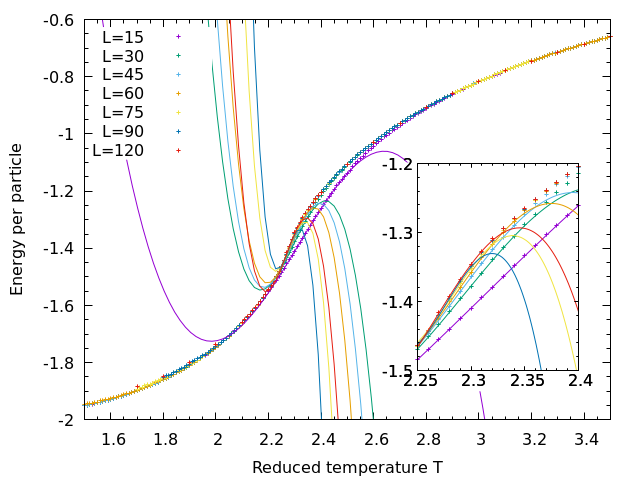
\includegraphics[width=\textwidth]{plot-e-fit.png}
        \caption{Energia per partícula}
        \label{fig:fit-e}
    \end{subfigure}
    \begin{subfigure}{.4\textwidth}
        \centering
        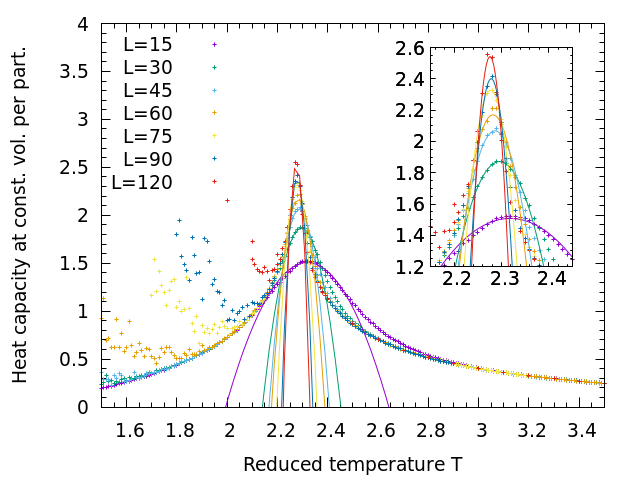
\includegraphics[width=\textwidth]{plot-cv-fit.png}
        \caption{Capacitat calorífica per partíucla}
        \label{fig:fit-cv}
    \end{subfigure}
        \begin{subfigure}{.45\textwidth}
        \centering
        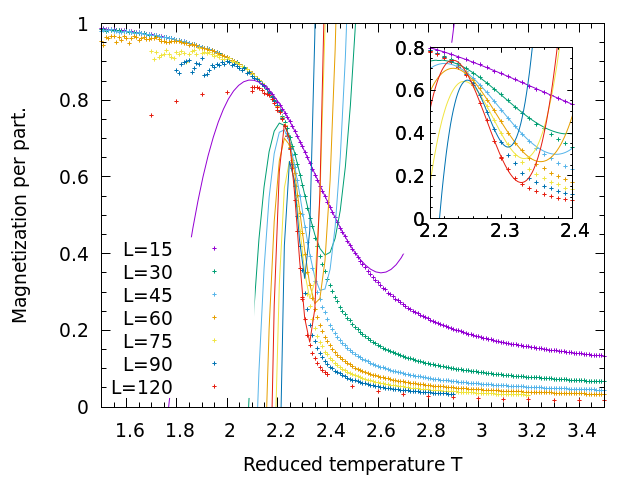
\includegraphics[width=\textwidth]{plot-m-fit.png}
        \caption{Imantació per partícula}
        \label{fig:fit-m}
    \end{subfigure}
    \begin{subfigure}{.45\textwidth}
        \centering
        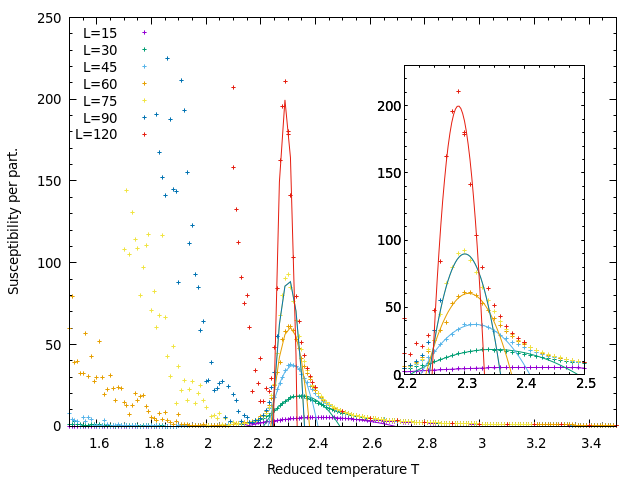
\includegraphics[width=\textwidth]{plot-x-fit.png}
        \caption{Susceptibilitat per partícula}
        \label{fig:fit-x}
    \end{subfigure}
    \caption{Figura \ref{fig:plot} a la qual s'hi han incorporat ajustos que descriuen les dades properes a la temperatura crítica: d'ordre 2 per a la capacitat calorífica i la susceptibilitat, i d'ordre 3 per a l'energia i la imantació.}
\label{fig:fit}
\end{figure}

\begin{table}[H]
\centering
\begin{tabular}{ccccc}
\hline
$\mathbf{L}$ & $\mathbf{T_c^e}$ & $\mathbf{T_c^{c_V}}$ & $\mathbf{T_c^m}$ & $\mathbf{T_c^\chi}$ \\ \hline
\textbf{15} & 2.31094 & 2.31828 & 2.35319 & 2.41181 \\
\textbf{30} & 2.29324 & 2.29584 & 2.30294 & 2.34911 \\
\textbf{45} & 2.28798 & 2.28633 & 2.29868 & 2.31780 \\
\textbf{60} & 2.28519 & 2.28208 & 2.29358 & 2.30702 \\
\textbf{75} & 2.28189 & 2.27703 & 2.28966 & 2.30240 \\
\textbf{90} & 2.27697 & 2.27836 & 2.28070 & 2.29320 \\
\textbf{120} & 2.26755 & 2.27569 & 2.27972 & 2.28713
\end{tabular}
\caption{Valors numèrics de les temperatures crítiques per a les diferents $L$ i les diferents propietats termodinàmiques. S'hi inclou una mitjana per cada $L$, en què es té en compte l'error estadístic.}
\label{tab:tcs}
\end{table}

Un cop tenim aquestes temperatures crítiques, en podem representar els comportaments amb l'invers de la longitud, per tal que l'ordenada a l'origen correspongui amb l'extrapolació al límit termodinàmic. No hi inclourem la temperatura crítica calculada en l'energia, ja que atès que la capacitat calorífica n'és la derivada, són formalment equivalents.
\begin{figure}[H]
    \centering
    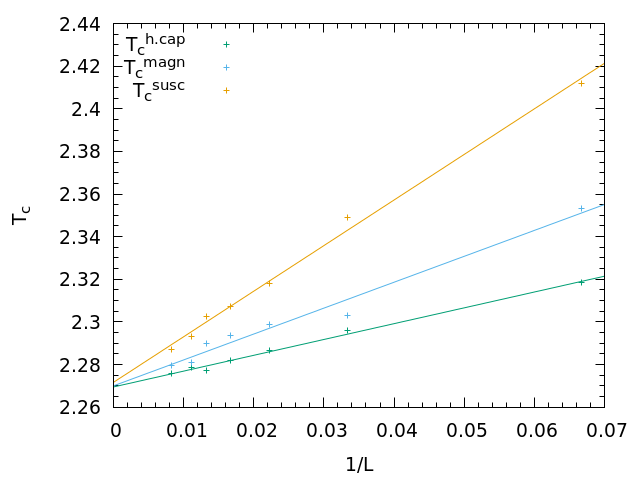
\includegraphics[width=.6\textwidth]{coefs-tc.png}
    \caption{Temperatures crítiques a $L$ finites. Es mostra la temperatura crítica contra $1/L$ i ajust lineal.}
    \label{fig:tc}
\end{figure}

Com diem, els ajustos de la figura \ref{fig:tc},
\begin{align*}
    T_c^{c_V} &= (0.74 \pm 0.02)/L + (2.2694 \pm 0.0008) \\
    T_c^{m} &= (1.22 \pm 0.09)/L + (2.270 \pm 0.003) \\
    T_c^{\chi} &= (2.14 \pm 0.07)/L + (2.271 \pm 0.002)
\end{align*}
tenen com a ordenada a l'origen la temperatura crítica que cadascuna de les magnituds termodinàmiques estudia.

Podem dir, doncs, que de manera conjunta, calculant-ne la mitjana i tenint en compte l'error estadístic:
\begin{equation} \label{t-mean}
    T_c = 2.2703 \pm 0.0011
\end{equation}
que està d'acord amb el valor teòric de la temperatura crítica:
\begin{equation*} \label{t-teo}
    T_c^\text{teo} = \frac{2}{\ln(1+\sqrt{2})} \approx 2.2692
\end{equation*}

\section{Exponents crítics}

Estudiem a continuació el comportament de les magnituds termodinàmiques prop de les temperatures crítiques. Sabem que ve donat pels exponents crítics:

\begin{equation*}
    \xi \propto \left| T-T_c \right|^{-\nu},\quad
    c_V \propto \left| T-T_c \right|^{-\alpha},\quad
    \chi \propto \left| T-T_c \right|^{-\gamma},\quad
    m \propto \left| T-T_c \right|^{\beta}
\end{equation*}

Podem considerar que al punt de temperatura crítica del sistema a $L$ finita, a què anomenarem $T_{cL}$,\footnote{N'hi ha una per a cada $L$ i cada magnitud termodinàmica. Són les que es presenten a la taula \ref{tab:tcs}.} té lloc un fenomen pseudocrític, on la correlació és màxima i proporcional a $L$. Sabent això,
\begin{align*}
    \xi &= A \left| T-T_c \right|^{-\nu} = KL \\
    \left|T_{cL}-T_c \right| &= \left(\frac{K}{A} L \right)^{-1/\nu} \\
    \ln \left(T_{cL} - T_c \right) &= -\frac{1}{\nu} \ln L + \text{const}
\end{align*}

Aleshores, n'hi haurà prou amb representar $\ln(T_{cL}-T_c)$ contra $\ln L$ i fer una regressió lineal (figura \ref{fig:coefs-nu}), i el valor de $\nu$ vindrà donat per l'invers del pendent amb el signe canviat. Això ho farem prenent les temperatures crítiques del sistema finit $T_{cL}$ obtingudes amb cadascuna de les propietats termodinàmiques, i la temperatura crítica obtinguda en l'extrapolació al sistema infinit $T_c$ presentada a l'equació \eqref{t-mean}.

Els ajustos trobats són els següents:
\begin{align*}
    \text{Capacitat calorífica:} &\quad \ln \left(T_{cL}^{c_V} - T_c\right) = (-1.09 \pm 0.08) \ln L + (0.0 \pm 0.3) \\
    \text{Imantació:} &\quad \ln \left(T_{cL}^{m} - T_c\right) = (-1.01 \pm 0.11) \ln L + (0.2 \pm 0.4) \\
    \text{Susceptibilitat:} &\quad \ln \left(T_{cL}^{\chi} - T_c\right) = (-1.02 \pm 0.04) \ln L + (0.87 \pm 0.16) \\
\end{align*}
que condueixen a uns valors de $\nu$:
\begin{align*}
	\nu_{c_V} &= 0.92 \pm 0.07 \\
	\nu_m &= 0.99 \pm 0.10 \\
	\nu_\chi &= 0.97 \pm 0.04
\end{align*}

Prendrem com a valor final la mitjana dels resultats anteriors:
\begin{equation} \label{nu}
    \nu = 0.96 \pm 0.04
\end{equation}

\begin{figure}[H]
    \centering
    \begin{subfigure}{.45\textwidth}
        \centering
        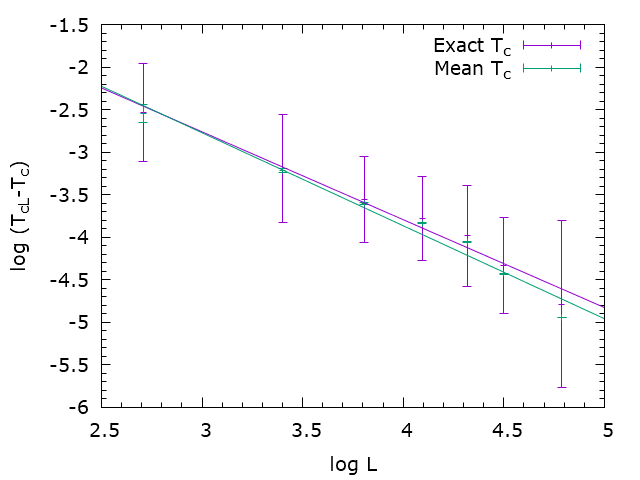
\includegraphics[width=\textwidth]{coefs-nu.png}
        \caption{Diferència de temperatures crítiques}
        \label{fig:coefs-nu}
    \end{subfigure}
    \begin{subfigure}{.45\textwidth}
        \centering
        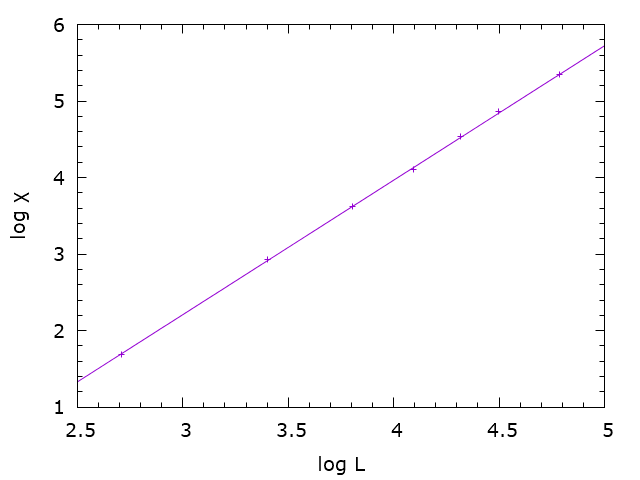
\includegraphics[width=\textwidth]{coefs-gammanu.png}
        \caption{Susceptibilitat}
        \label{fig:coefs-gammanu}
    \end{subfigure}
        \begin{subfigure}{.45\textwidth}
        \centering
        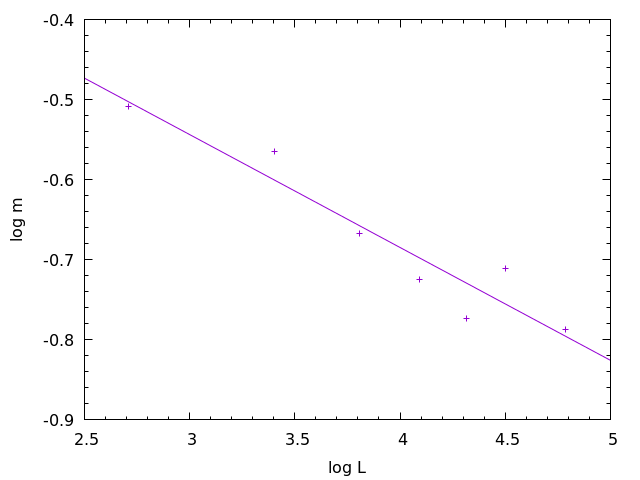
\includegraphics[width=\textwidth]{coefs-betanu.png}
        \caption{Imantació}
        \label{fig:coefs-betanu}
    \end{subfigure}
    \begin{subfigure}{.45\textwidth}
        \centering
        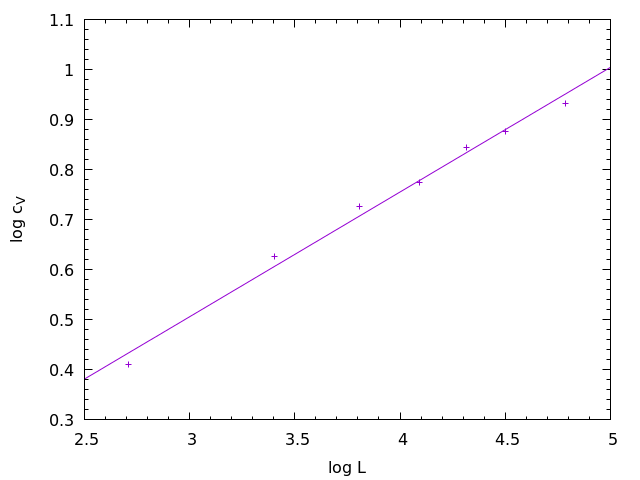
\includegraphics[width=\textwidth]{coefs-alphanu.png}
        \caption{Capacitat calorífica a volum constant}
        \label{fig:coefs-alphanu}
    \end{subfigure}
    \caption{Logaritme de les diferents magnituds termodinàmiques per partícula contra el logaritme de la longitud del costat de la matriu d'spins, amb els corresponents ajustos lineals. La figura \ref{fig:coefs-nu} mostra la diferència de la temperatura crítica en $L$, calculada per a cadascuna de les diferents magnituds termodinàmiques, amb la temperatura crítica per un sistema infinit calculada segons la mitjana d'extrapolacions amb les diferents magnituds termodinàmiques.}
\label{fig:coefs}
\end{figure}

Vegem la susceptibilitat. Podem relacionar-la amb la longitud de correlació i el seu coeficient mitjançant:
\begin{align*}
	\chi &= C \left|T_{cL}-T_c\right|^{-\gamma} = C \left[ \left(\frac{K}{A} L \right)^{-1/\nu} \right]^{-\gamma} = C \left(\frac{K}{A} L \right)^{\gamma/\nu} \\
	\ln \chi &= \frac{\gamma}{\nu} \ln L + \text{const}
\end{align*}

L'ajust de la figura \ref{fig:coefs-gammanu} resulta:
\begin{equation*}
	\ln \chi_L = (1.757 \pm 0.010) \ln L + (-3.06 \pm 0.04)
\end{equation*}

Sabem que el pendent és $\gamma/\nu$. Per tant, tenint en compte el valor de $\nu$ que obteníem a \eqref{nu} i amb la propagació d'incerteses:
\begin{equation*}
	\gamma = 1.69 \pm 0.06
\end{equation*}

De manera completament anàloga amb la imantació i la capacitat calorífica, representats en les figures \ref{fig:coefs-betanu} i \ref{fig:coefs-alphanu}, obtenim uns ajustos
\begin{align*}
	\ln m_L &= (-0.14 \pm 0.02) \ln L + (-0.12 \pm 0.08) \\
	\ln ({c_V})_L &= (0.249 \pm 0.011) \ln L + (0.24 \pm 0.04)
\end{align*}

que condueixen a uns coeficients
\begin{equation*}
	\beta = 0.14 \pm 0.02, \quad \alpha = 0.239 \pm 0.019
\end{equation*}

Comparem els resultats que hem obtingut amb els valors teòrics dels coeficients crítics:
\begin{table}[H]
\centering
\begin{tabular}{ccc}
\hline
\textbf{} & \textbf{Obtingut} & \textbf{Teòric} \\ \hline
$\nu$ & 0.96 $\pm$ 0.04 & 1 \\
$\gamma$ & 1.69 $\pm$ 0.06 & 1.75 \\
$\beta$ & 0.14 $\pm$ 0.02 & 0.125 \\
$\alpha$ & 0.239 $\pm$ 0.019 & 0
\end{tabular}
\caption{Comparació dels valors obtinguts pels exponents crítics amb els teòrics corresponents.}
\label{tab:critexp}
\end{table}

Els valors de tots quatre coeficients descriuen el comportament de les seves respectives magnituds termodinàmiques en la zona propera al punt crític. Veiem que els resultats s'ajusten força bé als valors teòrics pel que fa a $\nu$, $\gamma$ i $\beta$. Per altra banda, per a $\alpha$ no és el cas. El valor teòric $\alpha=0$ és conseqüència que, en el límit termodinàmic, la divergència de la capacitat calorífica és logarítmica. No obstant, aquest resultat no pot obtenir-se amb el model que fem servir aquí, ja que això només podria ser conseqüència de que no hi hagués cap dependència de la capacitat calorífica amb la temperatura, cosa que és no certa per a $L$ finites.

\section{Finite size scaling}

El mètode del \textit{Finite size scaling} (FSS) proporciona una eina per a verificar la bondat dels coeficients crítics. La hipòtesi de què parteix és que una propietat termodinàmica per a un sistema infinit $P_\infty (t)$ \footnote{Aquí, $t$ és una coordenada reduïda de la temperatura: $t = \frac{T^* - T_c}{T_c}$} té una contrapartida pels sistemes finits $P_L (t)$ que es comporta com:
\begin{equation*}
    \frac{P_L(t)}{P_\infty (t)} = f_P \left(x(t) \right), \quad x(t) \equiv \frac{L}{\xi_\infty (t)}
\end{equation*}
Si $P_\infty (t)$ presenta una divergència com $t^{-\rho}$ al punt crític ($t \to 0$), $P_L (t)$, que no deixarà de ser analítica, podrà expressar-se com:
\begin{equation*}
    P_L (t) = A t^{-\rho}\left[ 1 + Bt + Ct^2 + \mathcal{O}(t^3) \right] f_P \left( \frac{L}{D t^{-\nu} \left[ 1 + Et + Ft^2 + \mathcal{O}(t^3) \right]} \right)
\end{equation*}
on tant $P_\infty (t)$ com $\xi_\infty (t)$ separen les parts analítiques de les divergències. $P_L (t)$, per analiticitat, haurà de poder-se desenvolupar per sèries de Taylor:
\begin{equation*}
    P_L (t) = P_L (0) + \left.\dv{P_L}{t} \right|_{t=0} t + \frac{1}{2} \left.\dv[2]{P_L}{t} \right|_{t=0} t^2 + \mathcal{O}(t^3)
\end{equation*}

Calculant-se els coeficients i imposant-ne l'analicitat de cadascun d'ells es pot trobar la forma funcional de les derivades $f_P (x)$ i la dependència de cadascun dels termes amb $L$.
\begin{align*}
    \lim_{t \to 0} A t^{-\rho} f_P \left(\frac{L}{D} t^\nu \right) = \text{finit} \quad &\Rightarrow \quad f_P (x) \approx x^{\rho/\nu}, \quad P_L (0) \propto L^{\rho/\nu} \\
    \text{terme amb }\lim_{t \to 0} A t^{-\rho} f'_P \left(\frac{L}{D} t^\nu \right) \left[\frac{L}{D} \nu t^{\nu -1} \right] = \text{finit} \quad &\Rightarrow \quad \left.\dv{P_L}{t} \right|_{t=0} \propto L^{1/\nu} t \\
    \dots \quad &\Rightarrow \quad \left.\dv[2]{P_L}{t} \right|_{t=0} \propto L^{2/\nu} t^2 \\
    \text{etc.} &\ 
\end{align*}

De tal manera que, en global, pot escriure's com
\begin{equation} \label{eqpl}
    P_L (t) = L^{\rho/\nu} \left[p_0 + p_1 L^{1/\nu}t + p_2 L^{2/\nu}t^2 + \mathcal{O}(t^3) \right] \equiv L^{\rho/\nu} \psi_P(L^{1/\nu}t)
\end{equation}

Prendre com a magnitud termodinàmica $P_L$ la susceptibilitat, que divergeix com $\chi \propto t^{-\gamma}$, i la imantació que ---sense divergir--- es comporta com $\chi \propto t^{\beta}$ suposa fer canvis $\rho \leftrightarrow \gamma$ i $\rho \leftrightarrow -\beta$ en l'equació \eqref{eqpl}. Així doncs, si els coeficients $\nu$, $\gamma$ i $\beta$ són correctes, en representar $\langle |m_L| \rangle L^{\beta/\nu}$ en funció de $L^{1/\nu} (T^*-T_c)/T_c$ i $\langle \chi_L \rangle L^{-\gamma/\nu}$ en funció de $L^{1/\nu} (T^*-T_c)/T_c$ podem esperar que els punts col·lapsin en la mateixa corba prop del punt crític.

\begin{figure}[H]
    \centering
    \begin{subfigure}{.45\textwidth}
        \centering
        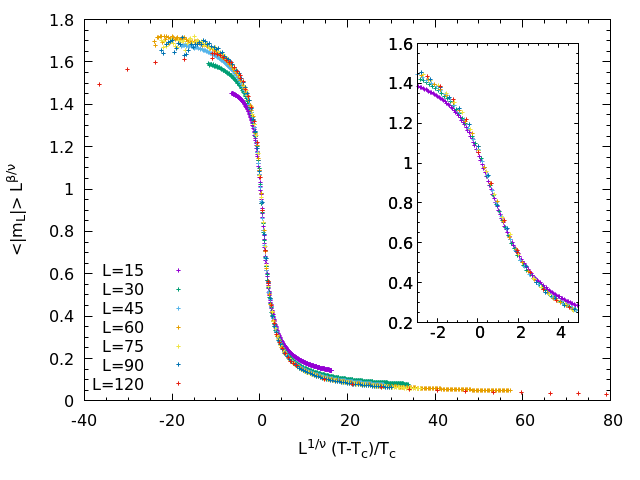
\includegraphics[width=\textwidth]{fss-m.png}
        \caption{Imantació}
        \label{fig:fss-m}
    \end{subfigure}
    \begin{subfigure}{.45\textwidth}
        \centering
        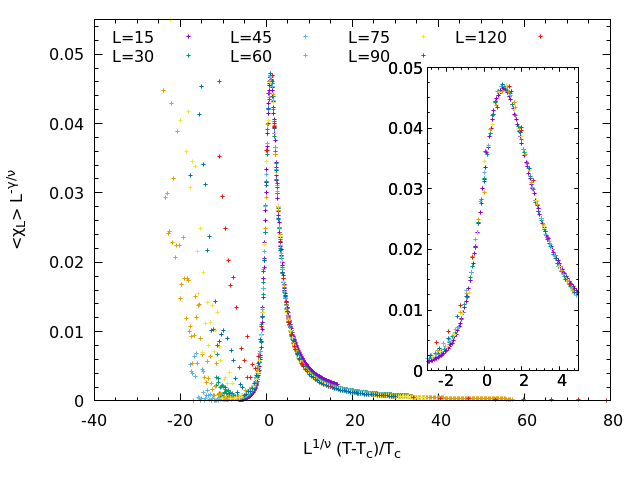
\includegraphics[width=\textwidth]{fss-x.png}
        \caption{Susceptibilitat}
        \label{fig:fss-x}
    \end{subfigure}
    \caption{Transformacions \textit{FSS} per a la imantació i la susceptibilitat.}
\label{fig:fss}
\end{figure}

\newpage
\section{Conclusions}
Al llarg del treball hem descrit quantitativament el comportament d'un sòlid paramagnètic mitjançant el model d'Ising bidimensional, tot explicant-ne les dependències de l'energia, capacitat calorífica, imantació i susceptibilitat amb la temperatura i el tamany i hem pogut observar com els comportaments s'ajustaven a les prediccions teòriques. A més, n'hem estudiat la criticalitat, de tal manera que hem estat capaços de trobar la temperatura crítica del sistema en el límit termodinàmic i els exponents crítics de les mateixes propietats termodinàmiques.

Els resultats obtinguts,
\begin{equation*}
    T_c = 2.2703 \pm 0.0011, \qquad \nu = 0.96 \pm 0.04, \qquad \gamma = 1.69 \pm 0.06, \qquad \beta = 0.14 \pm 0.02
\end{equation*}
Les discrepàncies i les incerteses han quedat sempre limitades pel rendiment de l'ordinador amb què les simulacions s'han dut a terme i el fet de disposar d'un temps de computació fitat. Això també pot apreciar-se a la figura \ref{fig:plot}, que presenta comportaments erràtics de les magnituds termodinàmiques a baixes temperatures per a $L$ altes. Tot i això, els resultats experimentals són prou bons, i en són prova el fet que en tots els casos les incerteses engloben els valors teòrics i la prova de \textit{finite size scaling}, on una transformació apropiada que involucra els propis valors obtinguts col·lapsa en una corba única prop del punt crític.

\begin{thebibliography}{9}
\bibitem{1}
\textit{Guions de pràctiques de l'assignatura Fenòmens col·lectius i transicions de fase}. Eduard Vives. Física UB, curs 2019-20.

\bibitem{2}
Kim J. K. \textit{Application to Finite Scaling to Monte Carlo Simulations} Physical Review Letters, 12-70 (1993).

\bibitem{3}
Brézin E. \textit{An investigation to finite size scaling}. J. Physique, 43-15 (1982).

\bibitem{4}
Pathria R. K., Beale P. D. \textit{Statistical Mechanics}. Academic Press (2011).

\end{thebibliography}

\end{document}
